\section{Additional SD\,1.5 figures}
\label{app:sd15}

\begin{figure}[!htbp]
\centering
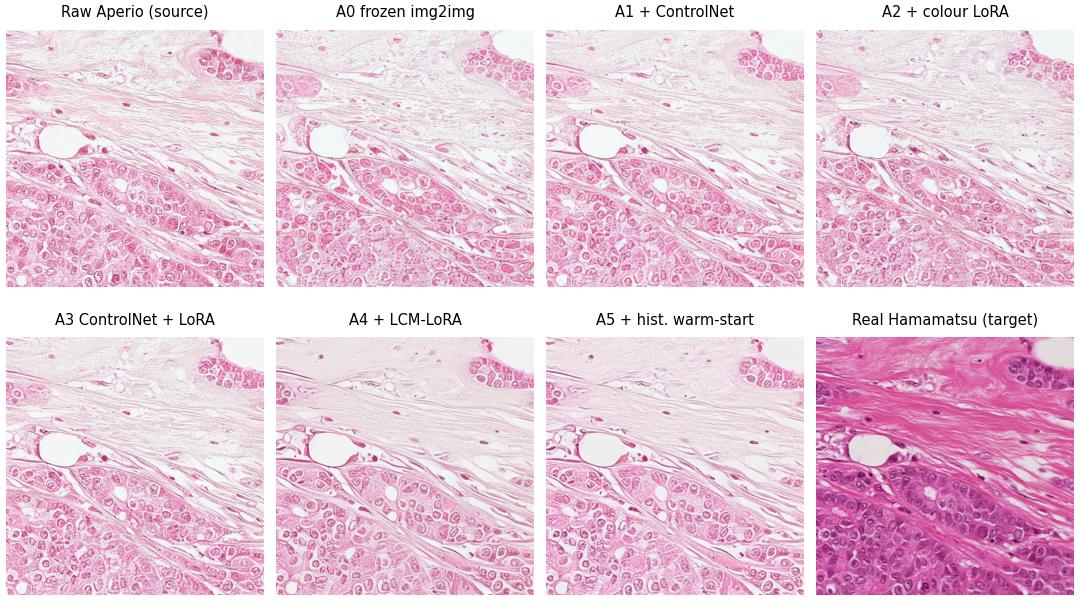
\includegraphics[width=0.62\textwidth]{ladder_grid_a06.jpg}
\caption{The A0--A5 ladder on the outlier slide A06 (strength 0.30). As on A08 (Fig.~\ref{fig:ladder}), no
rung approaches the target's colour.}
\label{fig:app-ladder}
\end{figure}

\begin{figure}[!htbp]
\centering
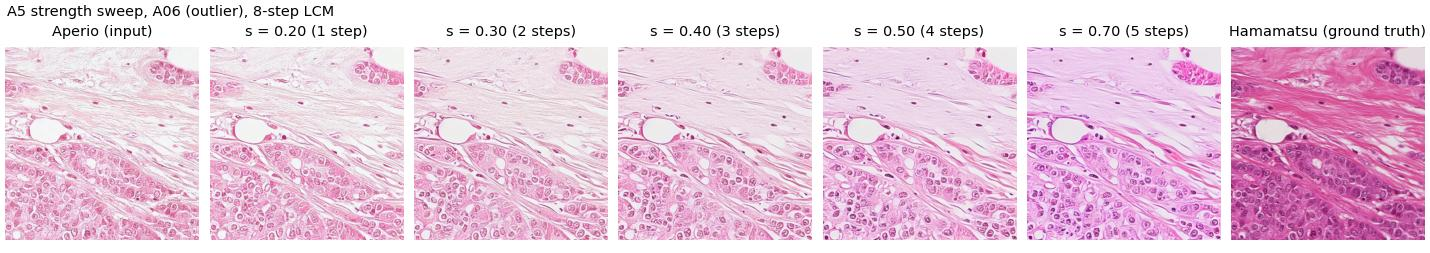
\includegraphics[width=\textwidth]{sweep_a5_06.jpg}\\[2pt]
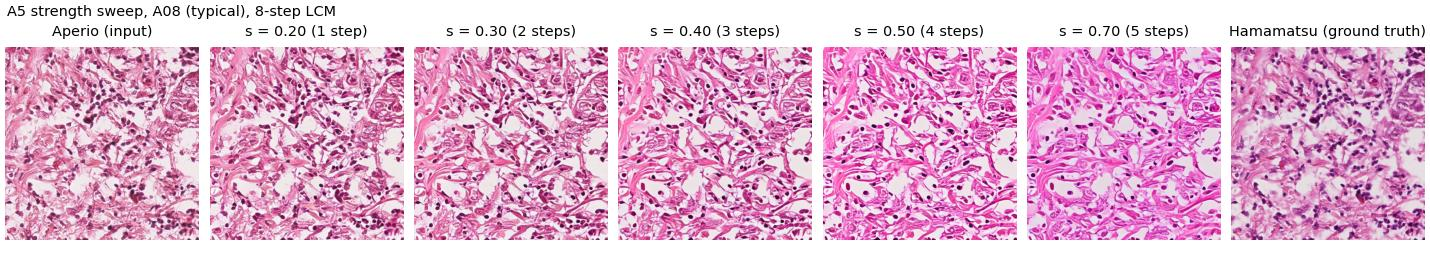
\includegraphics[width=\textwidth]{sweep_a5_08.jpg}
\caption{A5 strength sweep with 8 LCM steps on A06 (top) and A08 (bottom). Strength only sets how many steps
run ($\lfloor 8s\rfloor$). Colour moves towards the target on A06 as strength rises, while the typical slide
A08 loses both colour fidelity and structure.}
\label{fig:app-sweep}
\end{figure}

\begin{figure}[!htbp]
\centering
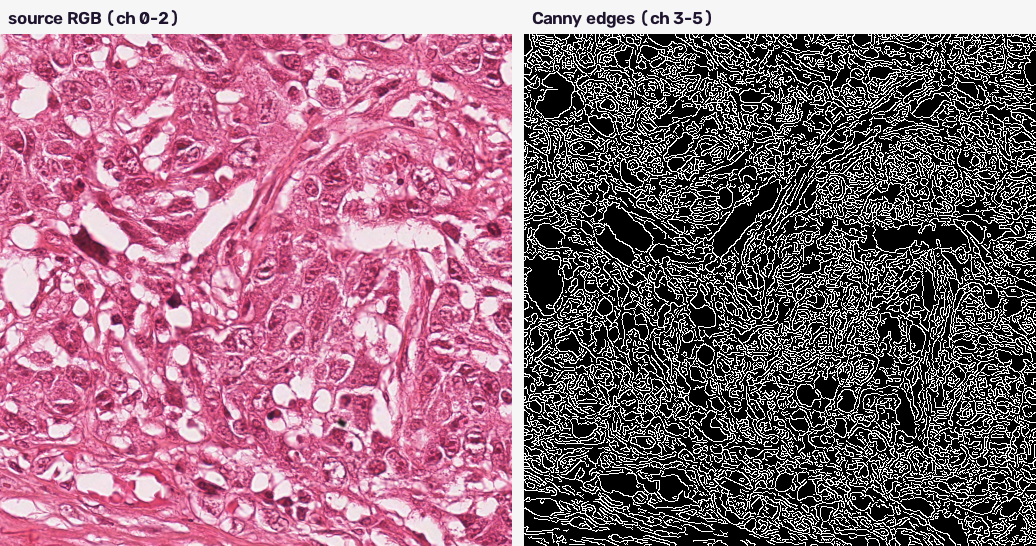
\includegraphics[width=0.42\textwidth]{controlnet_input.png}\hfill
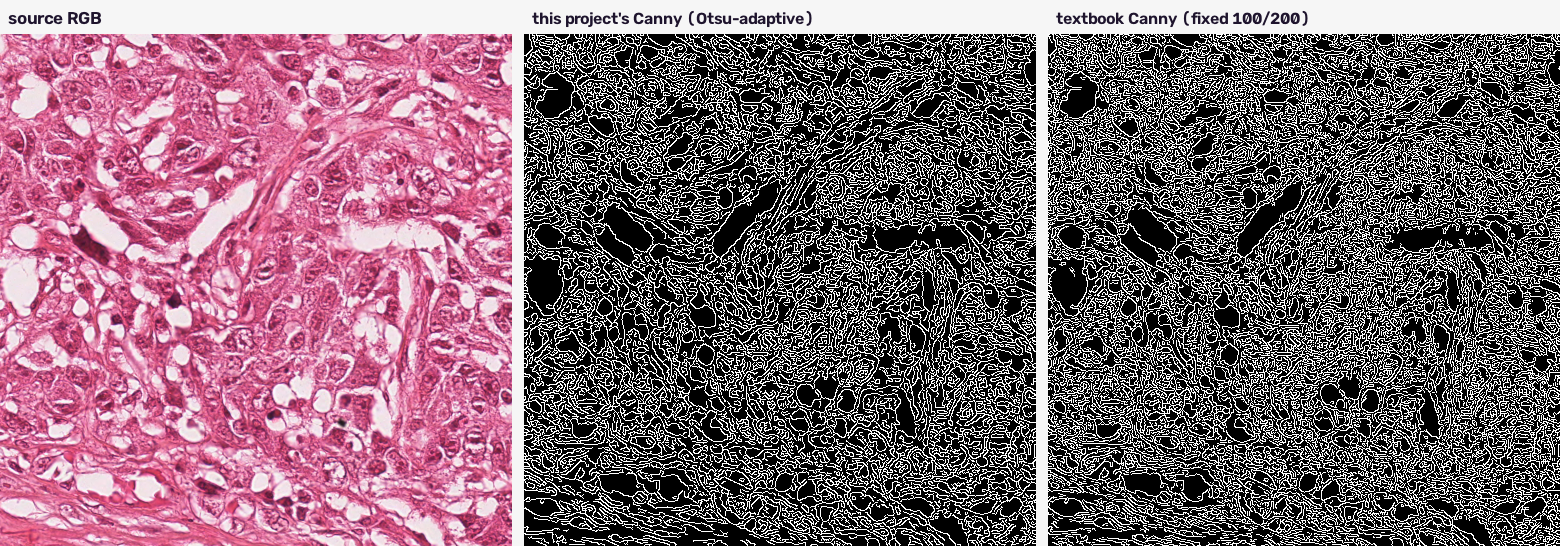
\includegraphics[width=0.56\textwidth]{controlnet_canny_comparison.png}
\caption{What the source-conditioned ControlNet sees (training crop A03\_00A). Left: the six-channel input,
source RGB and its Canny edges. Right: the source with our Otsu-adaptive Canny threshold and a fixed 100/200
threshold. Dense H\&E gives a busy edge map either way; the source RGB is the signal that lets the model learn
$p(H\mid A)$.}
\label{fig:app-controlnet}
\end{figure}

\begin{figure}[!htbp]
\centering
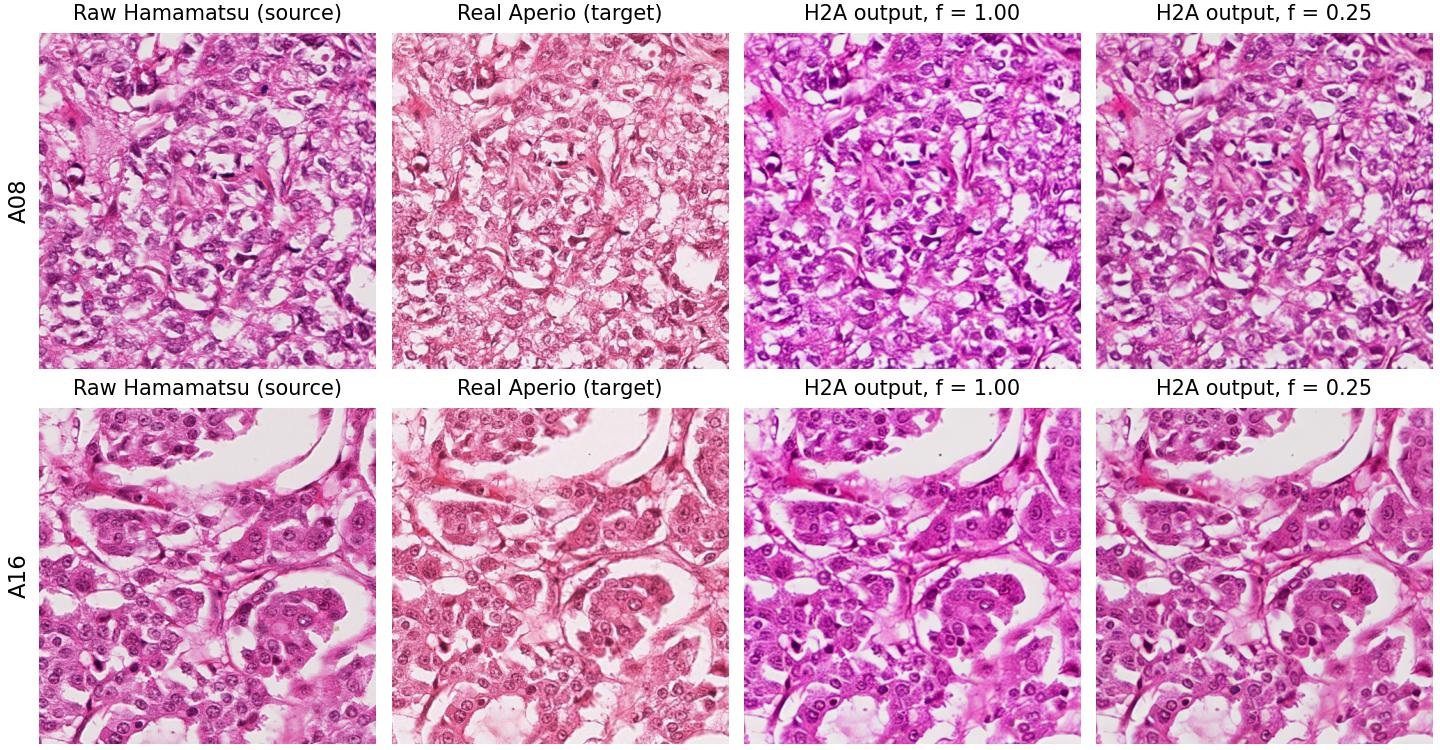
\includegraphics[width=0.72\textwidth]{p1_11_h2a.jpg}
\caption{SD\,1.5 in the \HtoA{} direction on held-out crops from A08 (top) and A16 (bottom): raw Hamamatsu source, real Aperio target,
and DDIM-inversion outputs with inversion fraction $f=1.00$ and $f=0.25$. Both drift towards magenta instead
of the paler Aperio colour ($\dlab=-15.6$ and $-6.2$).}
\label{fig:app-h2a}
\end{figure}

\begin{figure}[!htbp]
\centering
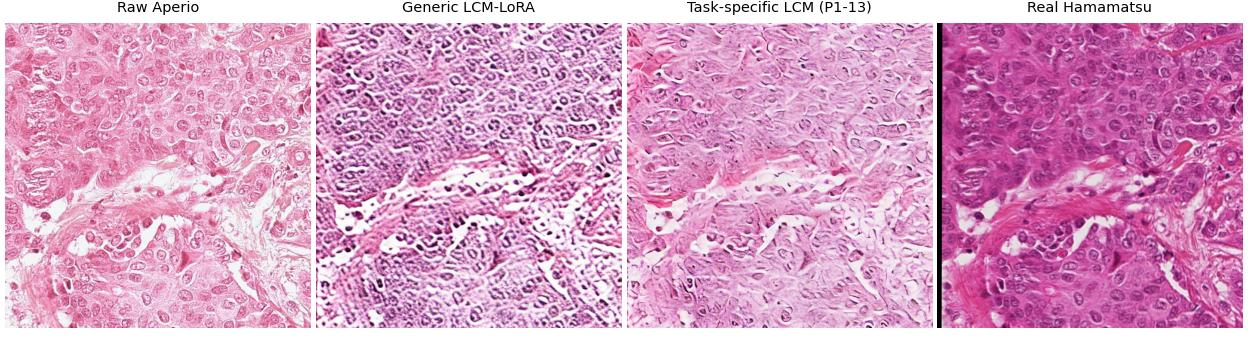
\includegraphics[width=0.8\textwidth]{p1_13_lcm.jpg}
\caption{Few-step inference on A06 (crop origin (0,0), seed 0): raw source, generic LCM-LoRA, the
task-specific distilled LCM, and the registered Hamamatsu target. Distillation did not improve on the generic
adapter.}
\label{fig:app-lcm}
\end{figure}

\begin{figure}[!htbp]
\centering
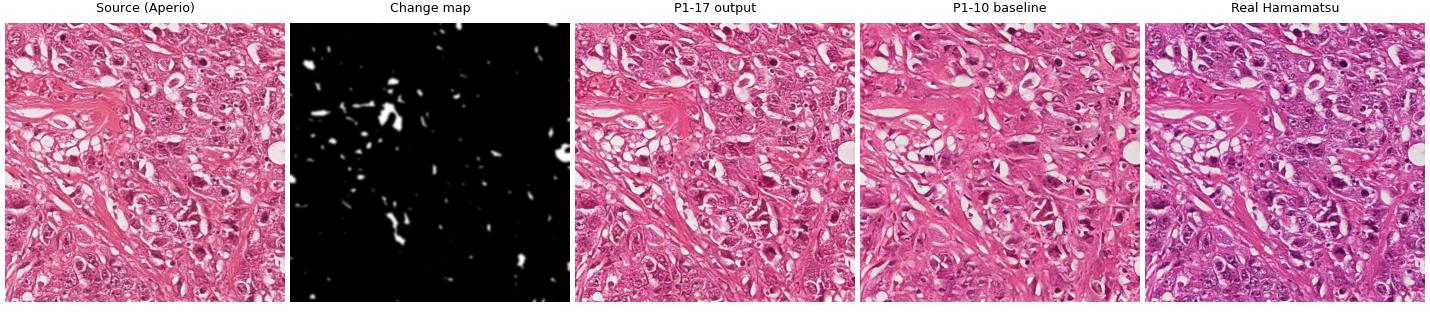
\includegraphics[width=0.9\textwidth]{p1_17_diffdiff.jpg}
\caption{Differential diffusion, a closed negative (training crop A03\_00A\_c024): source, the per-pixel change
map derived from edges, the differential-diffusion output, the plain source-conditioned baseline and the real
Hamamatsu crop. On dense H\&E the protected region covers nearly the whole crop, and SSIM did not change
(0.162--0.167 against $0.162\pm0.006$).}
\label{fig:app-diffdiff}
\end{figure}

\begin{figure}[!htbp]
\centering
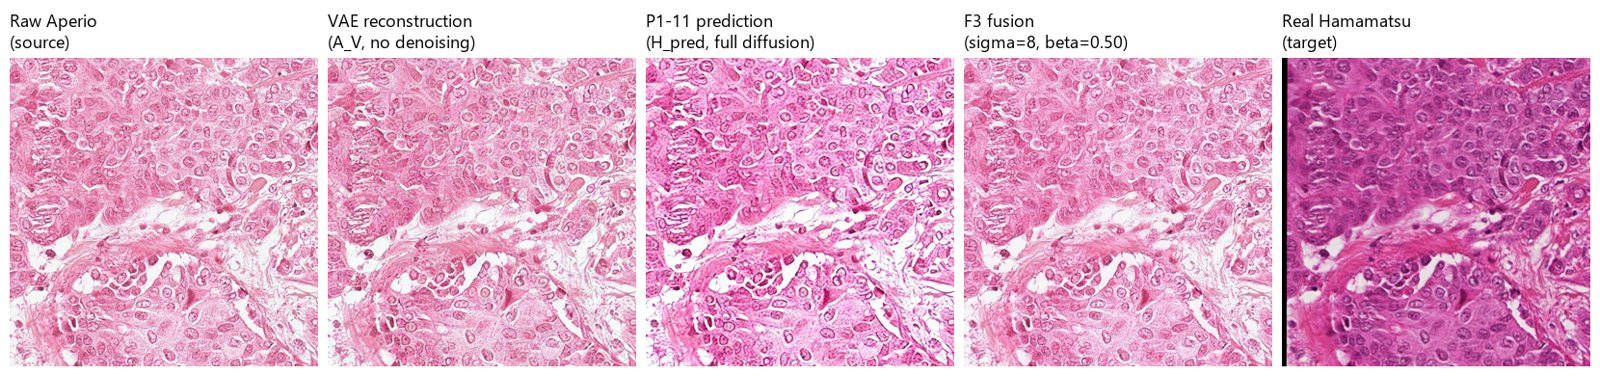
\includegraphics[width=\textwidth]{p1_16_a06.jpg}
\caption{F3 fusion on the outlier slide A06, laid out as Fig.~\ref{fig:f3}. The fused output keeps the source
structure but stays much paler than the Hamamatsu scan.}
\label{fig:app-f3}
\end{figure}

\begin{figure}[!htbp]
\centering
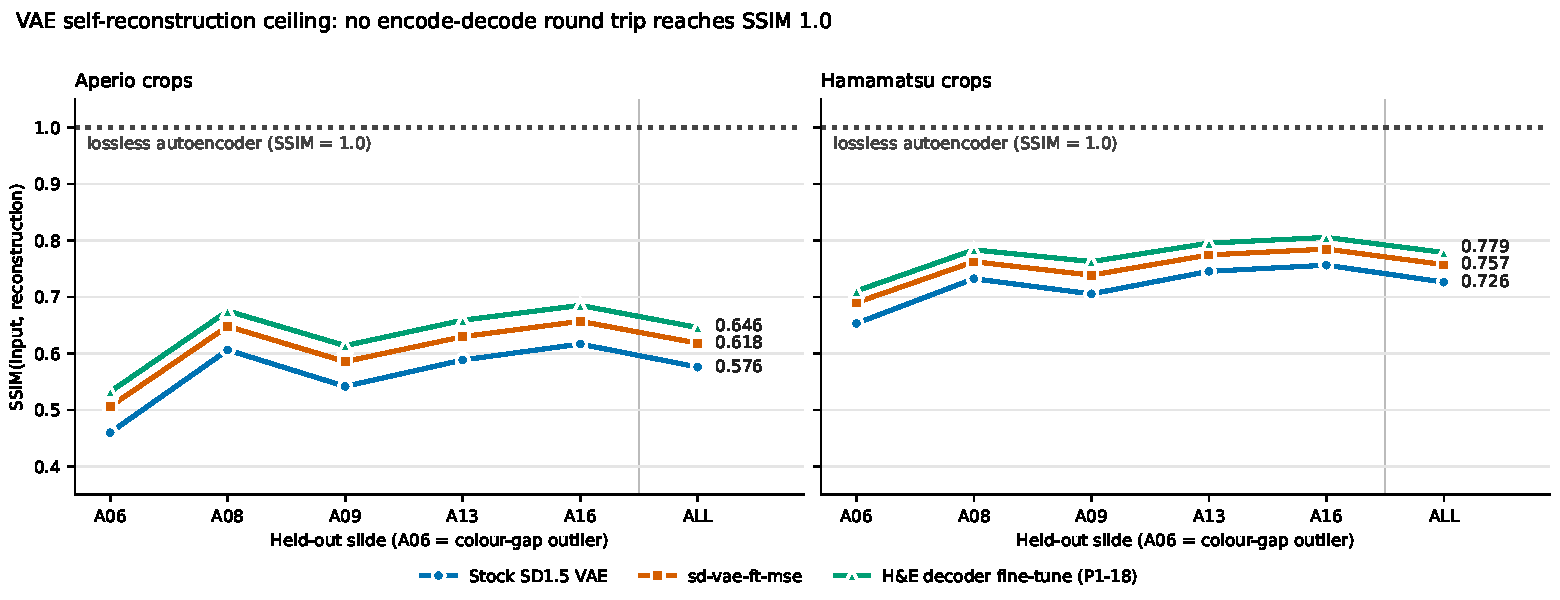
\includegraphics[width=0.9\textwidth]{vae_ceiling.pdf}
\caption{VAE self-reconstruction SSIM per held-out slide on Aperio (left) and Hamamatsu (right) crops, 496
crops each. The fine-tuned decoder is highest on every slide and every decoder stays far below the lossless
line (dotted).}
\label{fig:app-vae}
\end{figure}

\begin{figure}[!htbp]
\centering
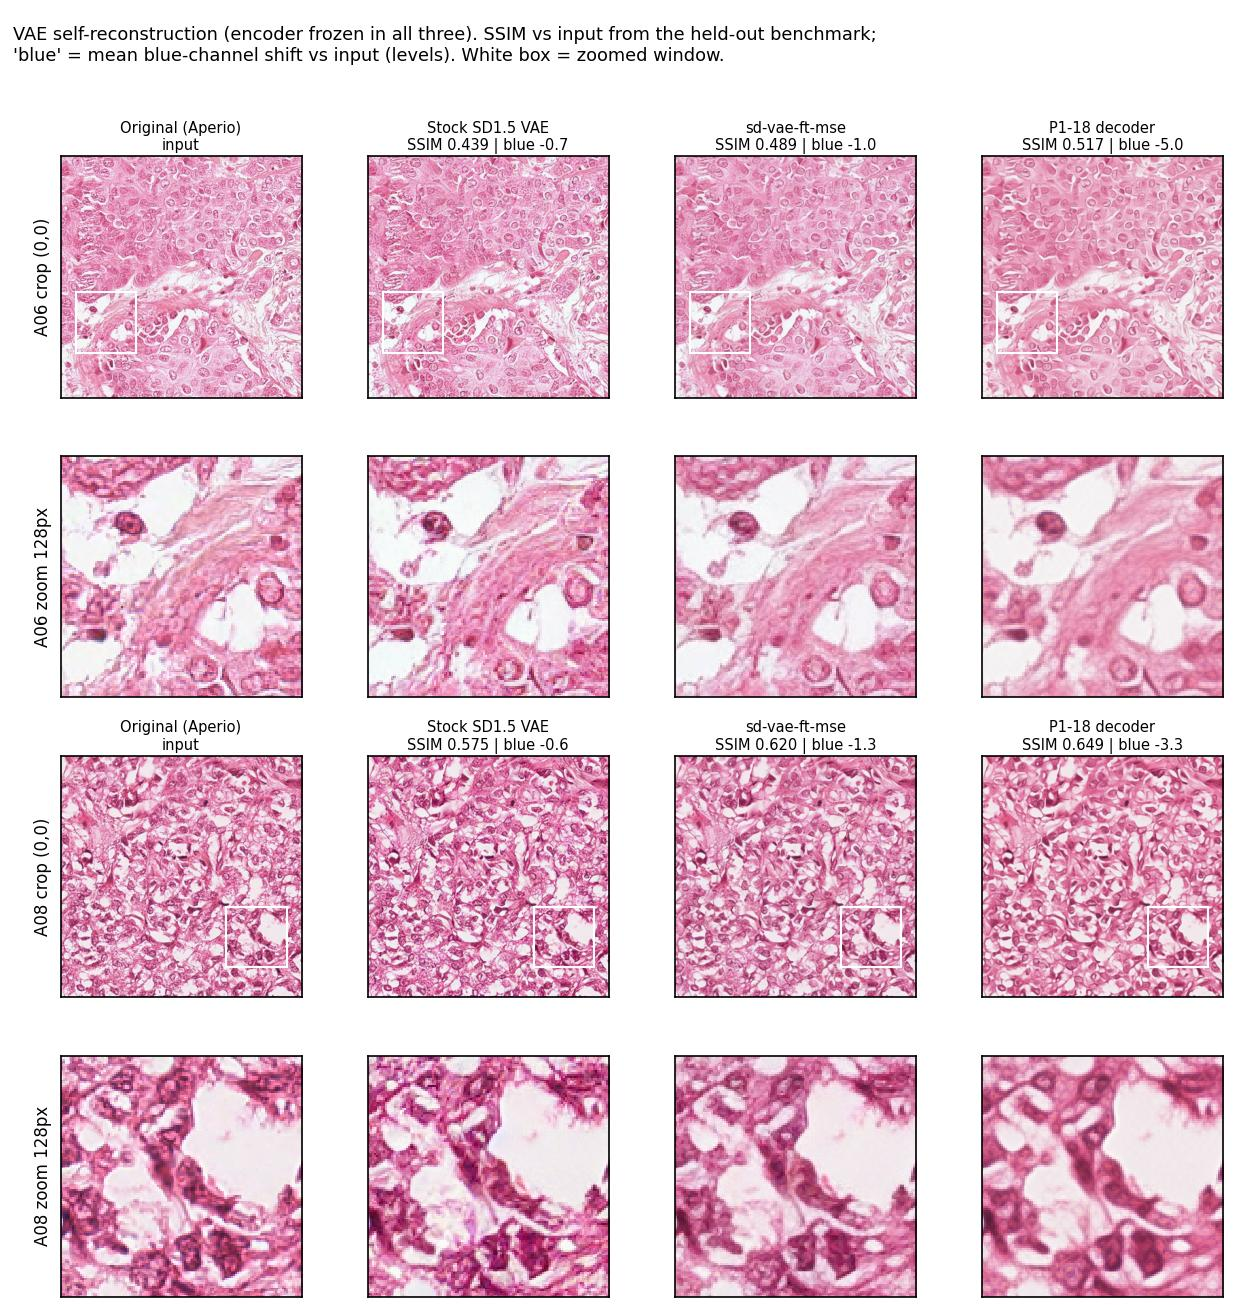
\includegraphics[width=0.47\textwidth]{p1_18_g12_recon.jpg}\hfill
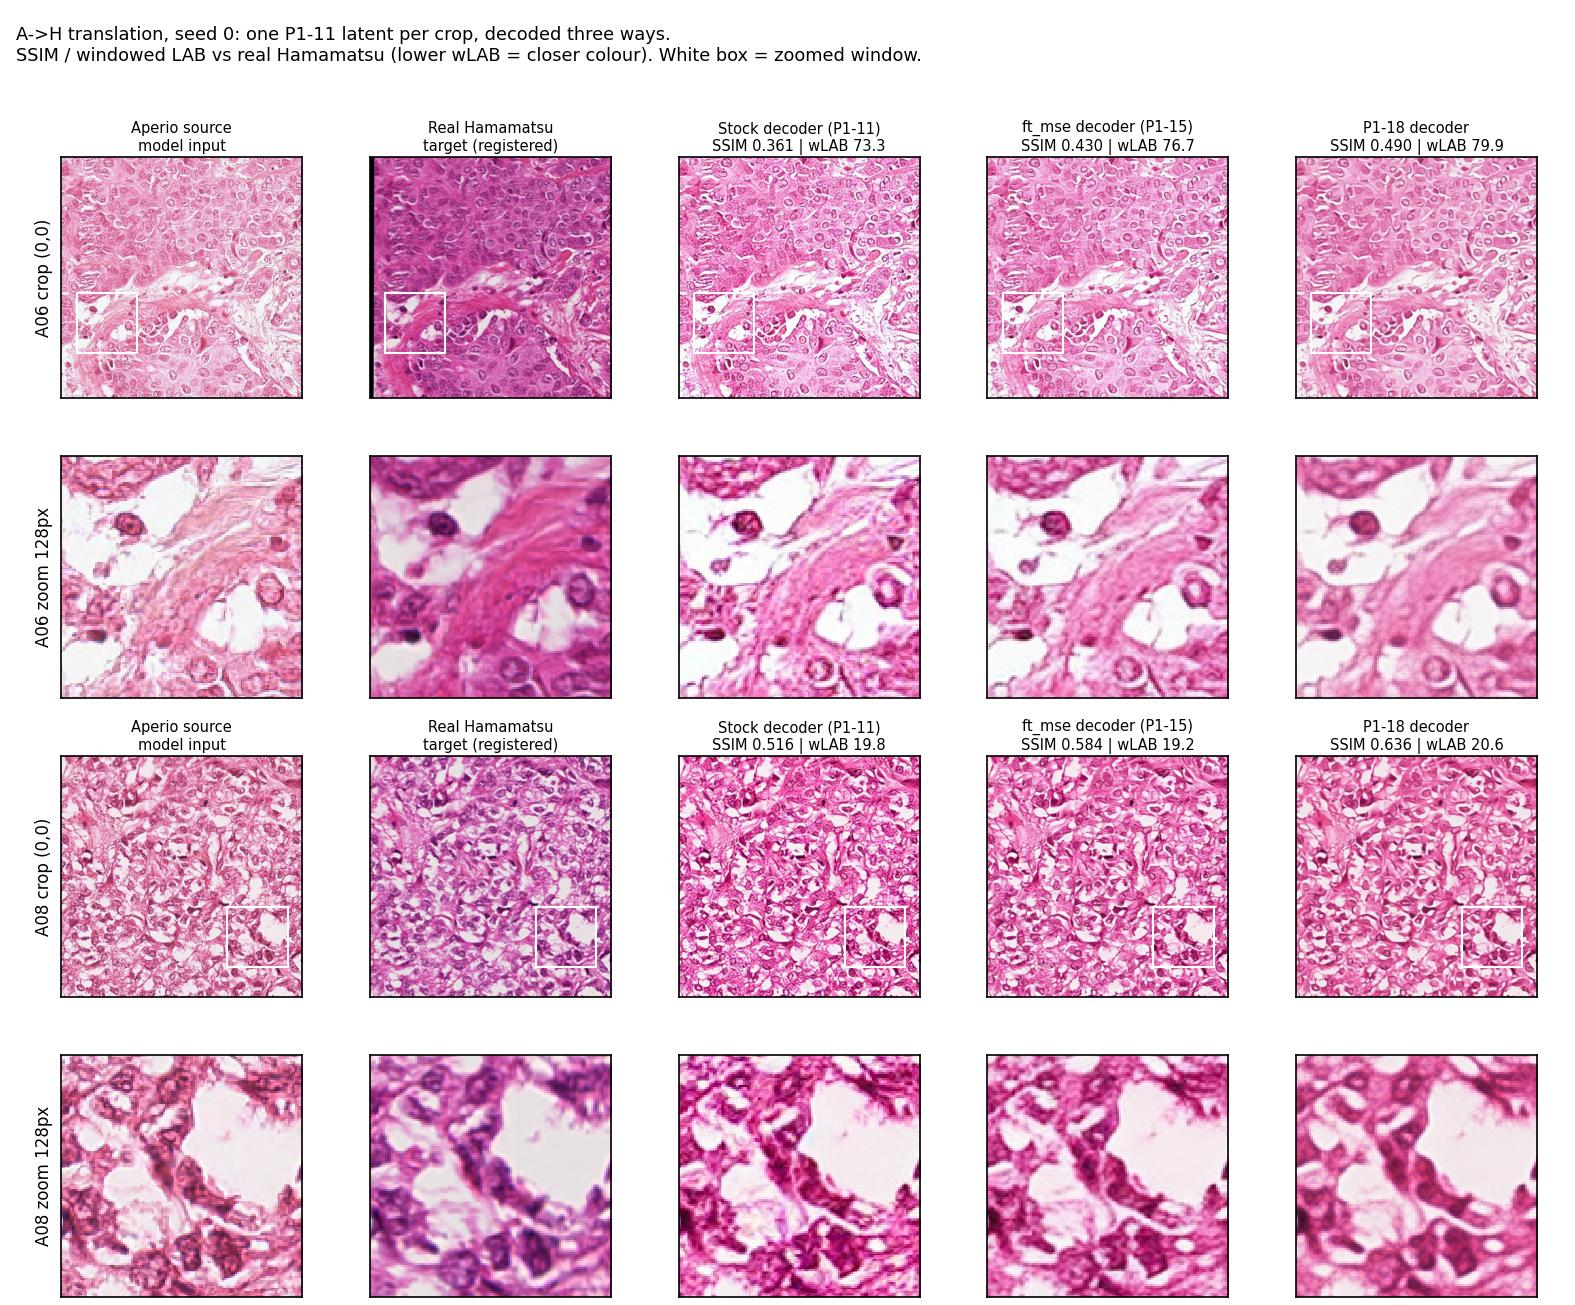
\includegraphics[width=0.52\textwidth]{p1_18_g12_translated.jpg}
\caption{Decoder comparison on A06 and A08, each with a 128\,px zoom. Left: self-reconstruction by the stock,
\texttt{ft-mse} and fine-tuned decoders, with SSIM and blue-channel shift against the input. Right: the same
DDIM-inversion latent decoded three ways, with SSIM and windowed LAB against the real Hamamatsu scan. The
fine-tuned decoder is the smoothest, which raises SSIM against the soft Hamamatsu target, and it shifts
colour slightly towards pink.}
\label{fig:app-decoder}
\end{figure}

\begin{figure}[!htbp]
\centering
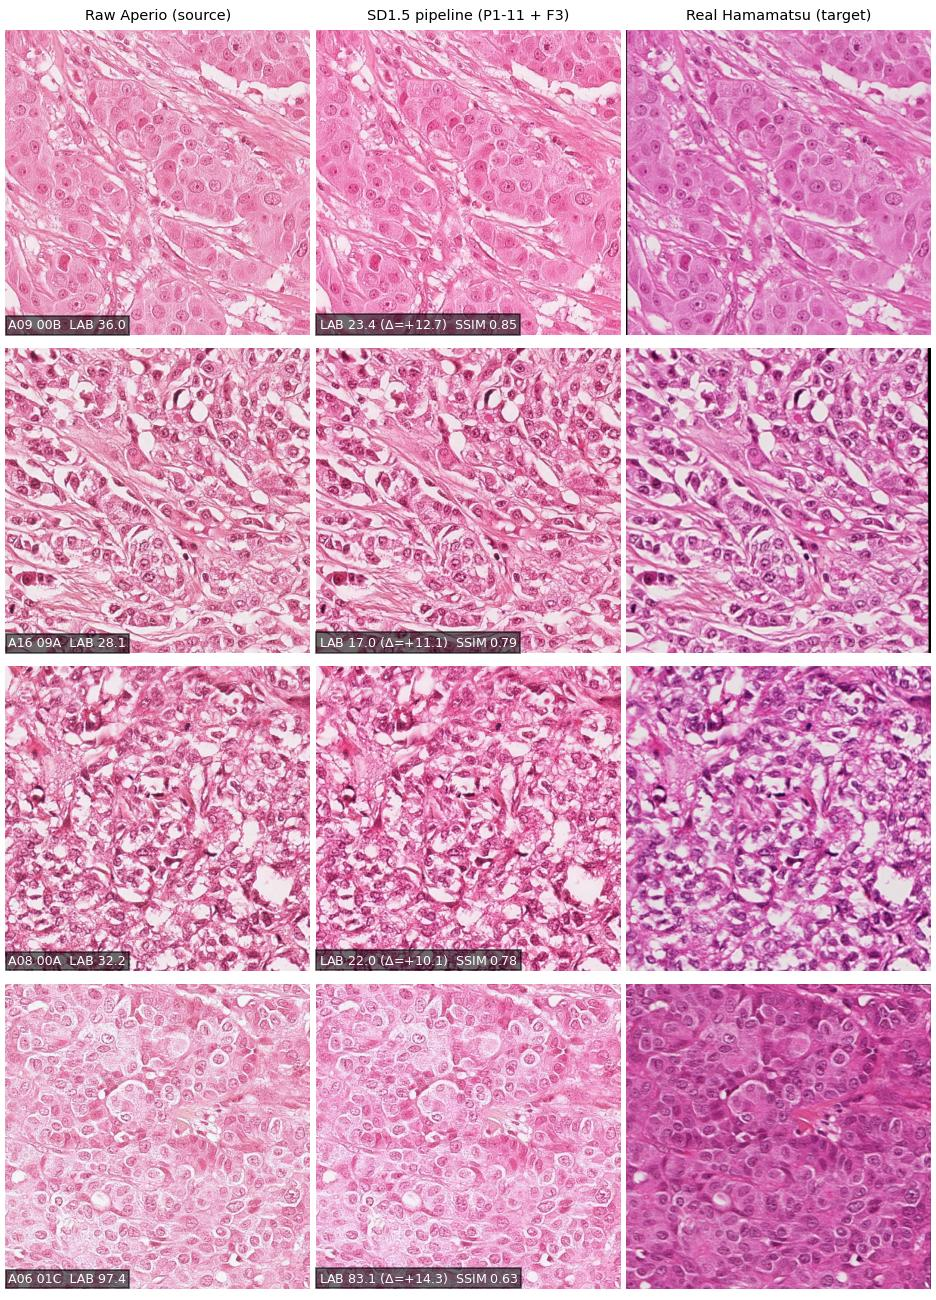
\includegraphics[width=0.46\textwidth]{best_cases_sd15.jpg}
\caption{Selected best cases of the final SD\,1.5 pipeline (DDIM inversion + F3 fusion): the top crop by
recovery on A09, A16, A08 and A06, with raw source, output and registered target. These are not typical: mean
recovery per slide is $+7.2$ to $+10.8$, and A06 stays paler than its target.}
\label{fig:app-best}
\end{figure}

\clearpage
\section{Evaluation figures}
\label{app:eval}

\begin{figure}[!htbp]
\centering
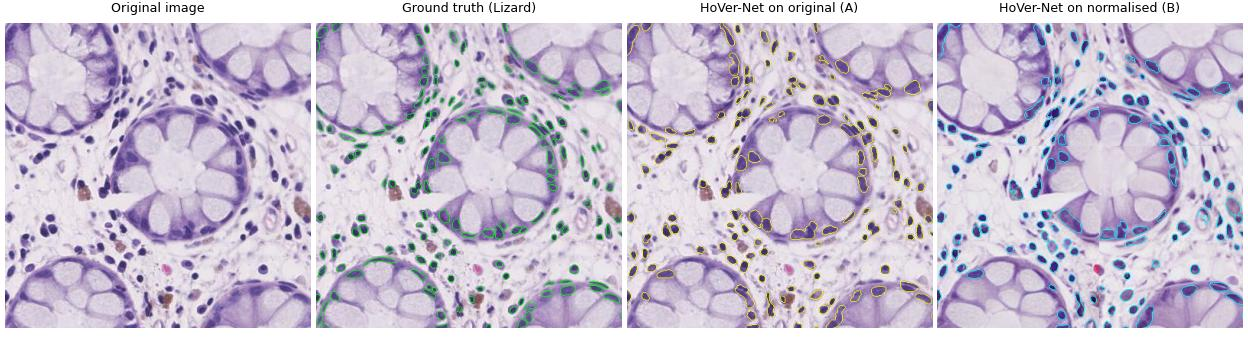
\includegraphics[width=0.8\textwidth]{lizard_overlay.jpg}
\caption{Structural-safety test on a typical Lizard image (400\,px patch; Dice(A,G) 0.741, Dice(B,G) 0.651,
ratio 0.878, the median): original, ground-truth nuclei, HoVer-Net on the original and on the normalised
image. HoVer-Net finds fewer nuclei after normalisation.}
\label{fig:app-lizard}
\end{figure}

\begin{figure}[!htbp]
\centering
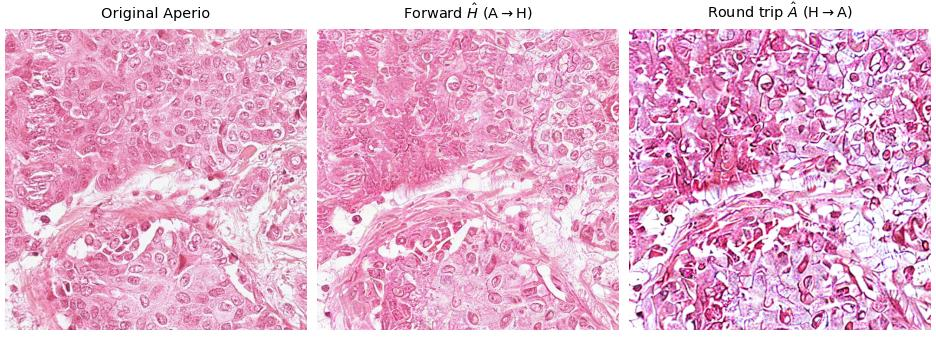
\includegraphics[width=0.62\textwidth]{roundtrip.jpg}
\caption{Round trip \AtoH{}\,$\to$\,A on A06 (50-step DDIM, strength 0.20): original, forward output and the
return trip. The return is oversaturated with distorted nuclear detail (SSIM 0.143 over 64 crops).}
\label{fig:app-roundtrip}
\end{figure}

\begin{figure}[!htbp]
\centering
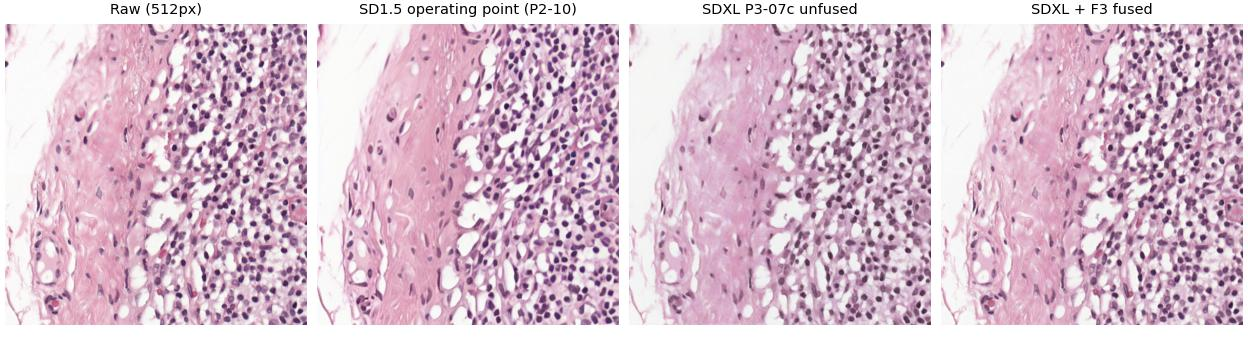
\includegraphics[width=0.85\textwidth]{camelyon_sdxl.jpg}
\caption{CAMELYON17 centre~0: raw patch, the SD\,1.5 operating-point output (the failed cross-centre test), and
the 144-pair SDXL model, unfused and with F3 fusion (run at 1024\,px).}
\label{fig:app-camelyon}
\end{figure}

\clearpage
\section{SDXL and probe figures}
\label{app:sdxl}

\begin{figure}[!htbp]
\centering
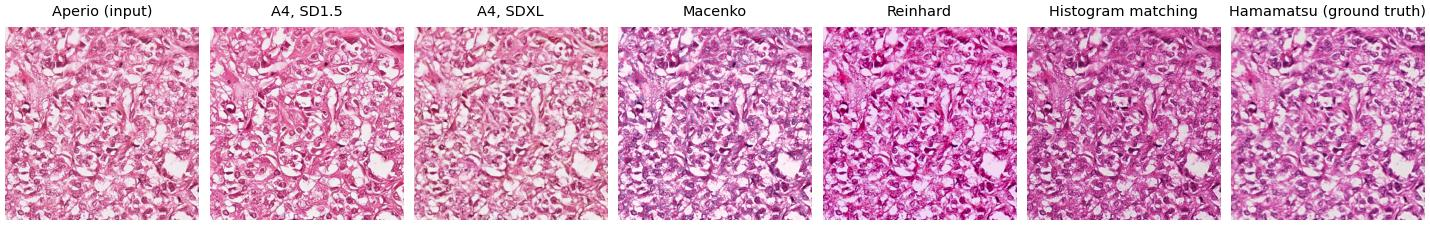
\includegraphics[width=\textwidth]{sdxl_vs_sd15.jpg}
\caption{A08 at the A4 configuration (strength 0.20) on SD\,1.5 and SDXL, with the classical baselines and the
real Hamamatsu scan.}
\label{fig:app-sdxl-sd15}
\end{figure}

\begin{figure}[!htbp]
\centering
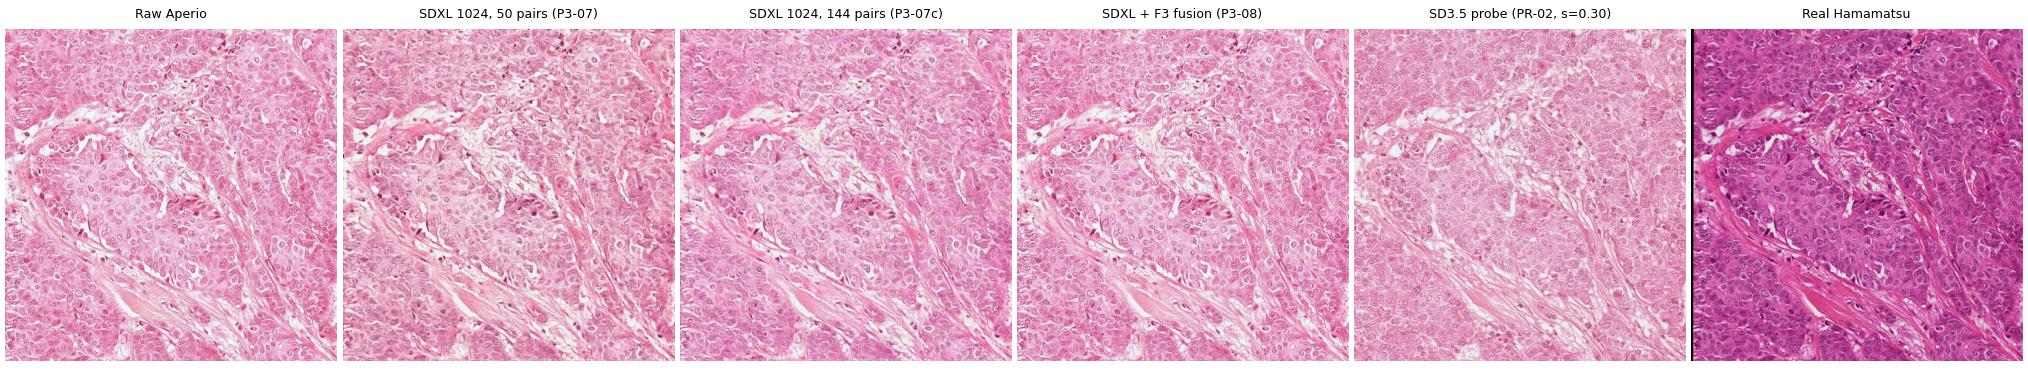
\includegraphics[width=\textwidth]{sdxl_sd35_panel_a06.jpg}
\caption{One 1024\,px A06 crop across methods, including the SD\,3.5 probe output (strength 0.30). The 50-pair
SDXL output stays near the Aperio colour, the 144-pair output is slightly more saturated, F3 fusion restores
source detail, and SD\,3.5 is washed out. The black strip on the Hamamatsu tile is registration padding.}
\label{fig:app-sd35}
\end{figure}

\begin{figure}[!htbp]
\centering
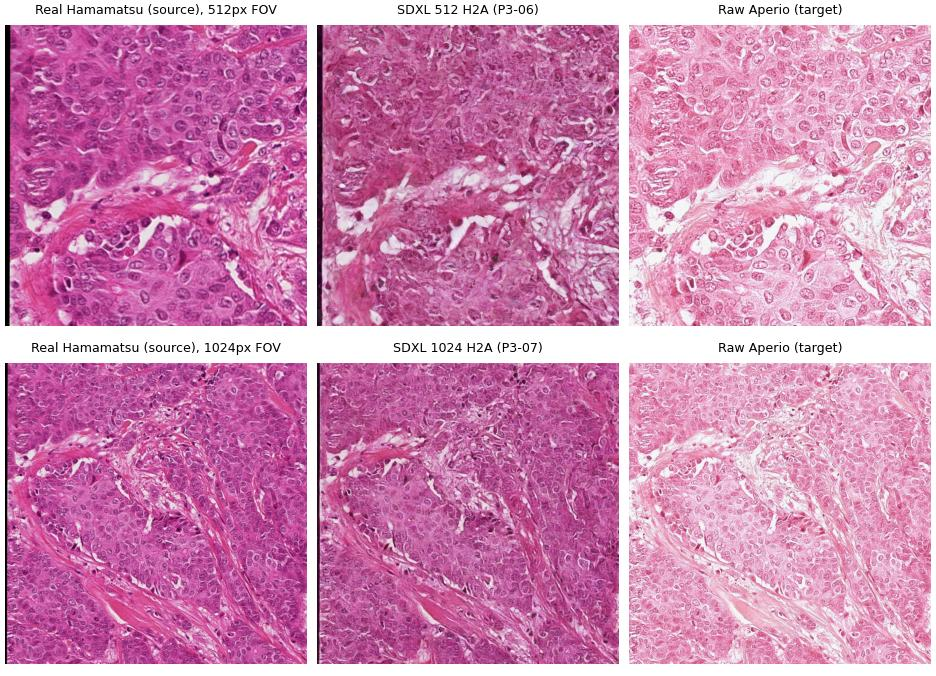
\includegraphics[width=0.6\textwidth]{sdxl_h2a.jpg}
\caption{SDXL \HtoA{} on A06 at 512\,px (top) and 1024\,px (bottom): real Hamamatsu source, SDXL output and raw
Aperio target. On this crop both outputs stay closer to the source than to the pale target; the mean
recoveries are $+9.47$ and $+9.20$.}
\label{fig:app-sdxl-h2a}
\end{figure}

\begin{figure}[!htbp]
\centering
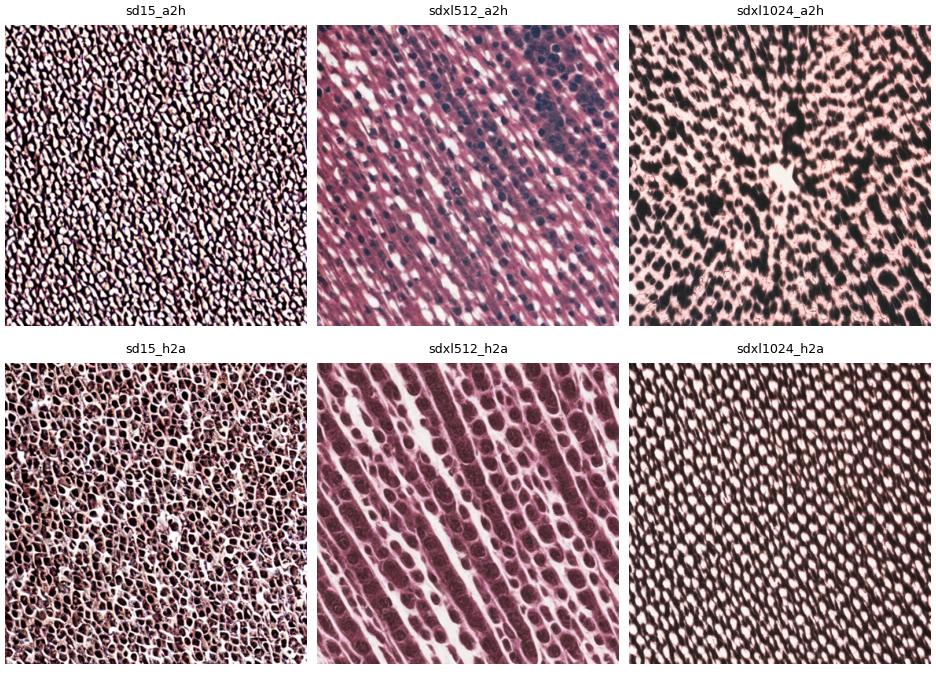
\includegraphics[width=0.6\textwidth]{t2i_backbones.jpg}
\caption{Pure text-to-image samples (seed 0) from SD\,1.5, SDXL at 512\,px and SDXL at 1024\,px, used only to
read each backbone's default colour in a diagnostic of the \AtoH{}/\HtoA{} asymmetry. They are repetitive
textures, not realistic tissue.}
\label{fig:app-t2i}
\end{figure}

\begin{figure}[!htbp]
\centering
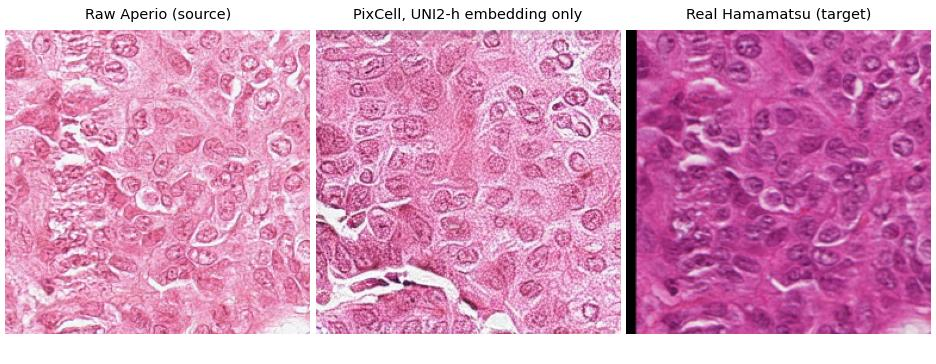
\includegraphics[width=0.62\textwidth]{pixcell_floor.jpg}
\caption{PixCell generation without fine-tuning from the crop's own UNI2-h embedding (A06, frame 00A, 256\,px).
The output is plausible H\&E tissue, but nuclei and glands are not where they are in the source or target
(SSIM 0.045).}
\label{fig:app-pixcell}
\end{figure}
